\scanpage{115}
\diagram{\begin{tikzcd}[ampersand replacement=\&,row sep=.6em,column sep=.5em]
 \&P_3\&\&\&\&\&\&x_1\\
 \&\Gamma\arrow[u]\arrow[dl]\arrow[dr]\&\&\&P_1\times P_2\arrow[dl]\arrow[dr]\&\&
 {(x_1,x_2)}\arrow[ur,"\sim"]\arrow[dr,dash,"\sim"']\&\\
 P_1\&\&P_2\&\underset{a_1}{P_1}\&\&\underset{a_2}{P_2}\&\&x_2
\end{tikzcd}}
\diagram{\begin{tikzcd}[ampersand replacement=\&,row sep=.2em,column sep=.8em]
 \&{(x_1,x_2)}\arrow[rr,"\sim"]\arrow[dl,"\sim"']\arrow[dd,"\unsure{2|\sim|\wr}"]\&\&{(a_1,x_2)}\arrow[dl,dash]\arrow[dd,"\unsure{2|\sim|\wr}"]\\
 x_1\arrow[dd,equal]\&\&x_2\&\\
 \&{(x_1,a_2)}\arrow[dl,"\sim"']\arrow[rr,"\sim"]\&\&{(a_1,a_2)}\\
 x_1\&\&\&
\end{tikzcd}}
\diagram{\begin{tikzcd}[ampersand replacement=\&,row sep=.5em,column sep=1em]
 \&\deleted{\unsure{Y}}X\times Y\arrow[dl]\arrow[dr]\&\\
 \underset{a}{X}\&\&\underset{b}{Y}
\end{tikzcd}}
\[
 x\xrightarrow[\sim]{\alpha_{x,y}}y\qquad
 \begin{aligned}x&\simeq b\\y&\simeq a\end{aligned}
 \qquad\begin{aligned}E_a&\simeq E_b\\\deleted{\unsure{E}}E_y&\simeq E_a\end{aligned}
 \qquad E_a\simeq E_b\simeq E
\]
\[
 \frac{\unsure{6|5|\Gamma}\cdot16\cdot2}{N}\qquad x\qquad
 \begin{aligned} E_x&\simeq E\\E_y&\simeq E\end{aligned}
\]
\[
\begin{aligned}
 &\alpha_{xy}^{*}:E\longrightarrow E\\
 &\unsure{\text{NB}|\text{où}|\text{avec}}\quad \alpha_{a,y}^{*}=\alpha_{a,b}^{*}=\mathrm{id}
\end{aligned}
\]
groupe libre \deleted{\unsure{non}} engendré par \(\alpha_{xy}^{*}\quad
(x,y)\in \deleted{\unsure{Y|X}}X\times Y-\deleted{\unsure{X}}\{a\}\times Y-\deleted{\unsure{Y|X}}X\times\{b\}\)

\[
\begin{aligned}
 X\times Y&\xrightarrow{\pi} Z\\
 E_{x,y}&\simeq E_{\deleted{\unsure{z}}\pi(x,y)}
\end{aligned}
\qquad
\begin{aligned}
 &\deleted{\unsure{xy}}\quad xy=x'y'=\pi\\
 &(e,\pi)\quad(\pi,e)\\
 &y=x^{-1}\pi\\
 &\deleted{\unsure{\in|\notin}}\quad x\ne e
\end{aligned}
\]
\[
 \underset{\substack{\Vert\\E}}{E_{e,\pi}}
 \overset{\varphi_{\pi;x}}{\simeq}
 \underset{\substack{\Vert\\E}}{E_{x,x^{-1}\pi}}
\]
\[
 \begin{aligned}
 &n^2-2n+1\\
 &{}+(n-1)n=\underbrace{2n^2-3n+1}
 \end{aligned}
 \qquad \gamma\in \Gamma\qquad 21\;/\;42
\]
\[
 \gamma\in \Gamma\qquad a_i\in P_i
\]
\figure{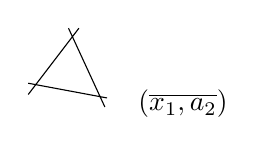
\begin{tikzpicture}[x=.55cm,y=.55cm]
 \draw (-.12,-.08)--(1.05,1.45) (.81,1.45)--(1.65,-.37) (-.12,.18)--(1.7,-.16);
 \node[anchor=west] at (2.2,-.3) {\((\overline{x_1,a_2})\)};
\end{tikzpicture}}
\[
 \underset{\substack{\Vert\\E_\gamma}}{E_{x_1}}\deleted{\simeq E_{x_2}}
\]
% archive sheet number: 116
